\documentclass{article}
\usepackage[table,xcdraw]{xcolor}
\usepackage{graphicx}
\usepackage{listings}
\usepackage{hyperref}
\usepackage{pdfpages}
\usepackage{csvsimple}
\usepackage{float}
\makeatletter
\newcommand\urlfootnote@[1]{\footnote{\url@{#1}}}
\DeclareRobustCommand{\urlfootnote}{\hyper@normalise\urlfootnote@}
\makeatother

\begin{document}
\title{Neural Networks Assignment 2}
\author{Group 35}
\maketitle
\lstset{
  basicstyle=\ttfamily,
  keywordstyle=\bfseries,
  language=Java,
  frame=single,
  aboveskip=11pt,
  belowskip=11pt,
  breaklines=true,
  breakatwhitespace=false,
  showspaces=false,
  showstringspaces=false,
  numbers=left,
  stepnumber=1,    
  firstnumber=1,
  numberfirstline=true
}

\section{Introduction}
This assignment is focused on getting familiar with the neural networks library \textit{Keras}\footnote{https://keras.io/ ; Visited 04.04.2018} written for \textit{python}\footnote{https://python.org/ ; Visited 04.04.2018}.
Section \ref{sec:mnist} focusses on using two different methods (MLP \& CNN) to classify handwritten digits taken from the MNIST-Dataset\footnote{http://yann.lecun.com/exdb/mnist/ ; Visited 04.04.2018}, asked for in the first part of assignment 2\footnote{See Slide 8 of "DeepLearning on GPUs.pdf"}.
Section \ref{sec:seq} is about natural language processing or the processing of arbitrary sequences / sentences,  required from the second part of assignment 2\footnote{See Slide 23 of "RecurrentNNs.pdf"}. This is done using LSTM's and GRU's instead of plain Recurrent Neural Networks (RNN's)
Section \ref{sec:rnn} then uses plain RNN's to see if based on pure sequence / string input it is possible to teach a neural network to do basic calculations like addition and multiplication.

\section{MNIST-Classification with Keras}
\label{task-1}
%xxxxxxxxxx – get them running
% xxxxxxxxx – print top 3 “most misclassified” digits
% xxxxxxxx – how do you define “most misclassified”? 
% xxxxxxxx change the error function to MSE and rerun your experiments
%– to which extent are your results reproducible? In other words:
%what is the impact of “non-controllable” randomness?
%xxxxxxxxx apply mnist_mlp.py and mnist_cnn.py to a “randomly permutedversion” of the mnist dataset (pixels of all images permuted with help of a fixed random permutation of their indices)


\label{sec:mnist}
This section is about the classification of handwritten digits using the MNIST-Dataset.
For this we used the existing \textit{keras}-example code called \texttt{mnist\_mlp.py}\footnote{\url{https://github.com/keras-team/keras/blob/master/examples/mnist_mlp.py} ; Visited 04.04.2018} and \texttt{mnist\_cnn.py}\footnote{\url{https://github.com/keras-team/keras/blob/master/examples/mnist_cnn.py} ; Visited 04.04.2018}. 
The existing code uses the \textit{cross-entropy error} function.

In order to see the impact of the error function we repeated the experiment using the \textit{mean-squared error} function.

We also wanted to test out what happens if we permutate both the training and test samples.
For each experiment we output the three most misclassified digits.
We define \textit{most misclassified} as follows: The samples where the probability of the $y_{true}$ label was the lowest.

\subsection{Evaluation}

In table \ref{table-1} you can see the amount of misclassified samples per experiment.
It is evident, that CNN outperforms the MLP.
Only with permuted data it has troubles.
The reason for that was explained in the section \ref{task-1}.
Both networks perform best with the cross-entropy error function.
The mean-squared error only slightly worsens the results of the MLP.
The CNN however, performs much worse using cross-entropy.

\begin{table}[]
	\centering
	\begin{tabular}{|l|l|l|l|l|}
		\hline
		& \cellcolor[HTML]{C0C0C0}CEE & \cellcolor[HTML]{C0C0C0}CEE-P & \cellcolor[HTML]{C0C0C0}MSE & \cellcolor[HTML]{C0C0C0}MSE-P \\ \hline
		\cellcolor[HTML]{C0C0C0}MLP & \cellcolor[HTML]{FFFFFF}166 & 178                           & 169                         & 189                           \\ \hline
		\cellcolor[HTML]{C0C0C0}CNN & 77                          & 123                           & 149                         & 221                           \\ \hline
	\end{tabular}
	\caption{Amount of misclassified samples. CEE = cross-entropy error; MSE = mean-squared error, P = permutated sample}
	\label{table-1}
\end{table}

Looking at figure \ref{fig:cnn} we can that the few misclassifications mostly seem to revolve around hardly digits.
The 9 is too thin, the 1 is barely visible and the 8 is too thin, too little and contains a noisy line.

\begin{figure}[H]
	\centering
	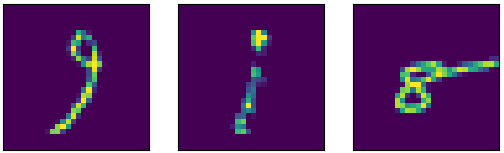
\includegraphics[width=0.5\linewidth]{img/cnn_categorial_cross_non_perm.png}
	\caption{Top three most misclassified digits with the CNN-CEE net}
	\label{fig:cnn}
\end{figure}


The three most misclassified digits of the MLP, shown in figure \ref{fig:mlp}, stand in stark contrast to that.
The left and the right sample seem to be very clearly identifiable.
One problem might be the thickness given that both samples are quite thick.
The third is easily identifiable by a human, but is very thin compared to the others, which probably is the reason why it was misclassified.
Of course other reasons could have led to this result as well.


\begin{figure}[H]
	\centering
	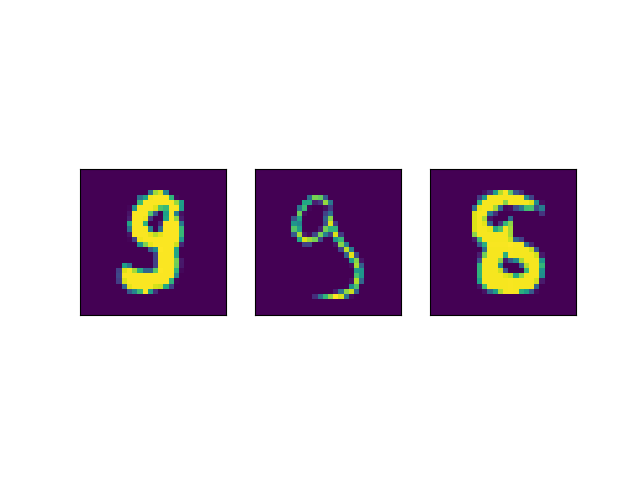
\includegraphics[width=0.5\linewidth]{img/mpl_categorial_cross_non_perm.png}
	\caption{Top three most misclassified digits with the MLP-CEE net}
	\label{fig:mlp}
\end{figure}


The convulationen is more affected that the MLP by permutation.
This is explainable by way of how a convulitional filter is working.
It looks at neighbouring pixels and summarizes them into a new value.
Of course a random permutation will influence these sums in an unpredictable way.
This results in a most grey filtered image, which is much harder to classify.
This doesn't apply to MLP, because every pixel considered without any modification.


\subsection{Randomness impact}
To determine the possible impact of randomness upon accuracy of the recognition we run same tests again.
Keras offers various weight initiliazers, these initial weights influence the training process and the final result.
This can be seen, if we compare table \ref{table-1} to table \ref{table-2}.
However, the margin between the misclassified samples seems negligible.


\begin{table}[H]
	\centering
	\begin{tabular}{|l|l|l|l|l|}
		\hline
		& \cellcolor[HTML]{C0C0C0}CEE & \cellcolor[HTML]{C0C0C0}CEE-P & \cellcolor[HTML]{C0C0C0}MSE & \cellcolor[HTML]{C0C0C0}MSE-P \\ \hline
		\cellcolor[HTML]{C0C0C0}MLP & \cellcolor[HTML]{FFFFFF}154 & 160                           & 169                         & 174                           \\ \hline
		\cellcolor[HTML]{C0C0C0}CNN & 88                          & 128                           & 147                         & 216                           \\ \hline
	\end{tabular}
	\caption{Amount of misclassified samples. CEE = cross-entropy error; MSE = mean-squared error, P = permutated sample}
	\label{table-2}
\end{table}

\section{Processing Sequences using LSTM's and GRU's}
\label{sec:seq}
This section deals with using LSTM's and GRU's for natural language processing.
It is split up into two parts one dealing with the generation of text (Section \ref{sec:gen}) based on the learned data and the one that handles the translation of text (Section \ref{sec:trans})
\subsection{Generating Text}
\label{sec:gen}
The text generation is based on the \textit{keras}-example code called \textit{lstm\_text\_generation.py}\footnote{\url{https://github.com/keras-team/keras/blob/master/examples/lstm_text_generation.py} ; Visited 04.04.2018}.
In order to evaluate the generation we run the following experiments
\begin{itemize}
\item{Run the example-script as is}
\item{Run the example with different text input}
\item{Run the example with different text input and adjusted parameters to the LSTM}
\item{Run the example with different text input and use a GRU instead of LSTM}
\end{itemize}


TODO: mention sliding window


Also the standard script uses a sequence length of 40 characters. We found that a little short. In order to find a good length we looked up the average sentence length in the english language which is supposed to be 15-20\footnote{\url{http://countwordsworth.com/blog/what-is-a-good-average-sentence-length/} ; Visited 04.04.2018}.
Also the average word length is approximately 5 characters\footnote{\url{https://www.quora.com/Whats-the-average-length-of-English-words} ; Visited 04.04.2018}. Combining that results in 100 characters per sentence ($20 * 5$). We also expect a longer sequence length to improve the generated result, given that LSTM's use historical data well, and short sequences might already have dropped relevant previous context\footnote{\url{http://colah.github.io/posts/2015-08-Understanding-LSTMs/}; Visited 04.04.2018}.

Running the vanilla example script generates very noisy text with a lot of new lines where they are not supposed to be. That is why we decied to write a cleaner for the custom text.

We chose to use all bands of harry potter which are available as txt files on archive.org.
It does contain "noise" in the sense of page numbers, titles which were misread due to ocr etc. We filtered this out with a script.
We also had a few problems with the script aborting due to non-ascii characters being contained in the text, hence we had to drop even more content from the file to work properly.

TODO: abschnitt long term dependencies. france beispiel erwähnen

\subsection{Translating Text}
\label{sec:trans}
\begin{itemize}
\item{Run the example-script as is with french to english translatoin}
\item{Run the example with NL-ENG input}
\item{Run the example with NL-ENG input and adjusted parameters to the LSTM}
\item{Run the example with NL-ENG input and use a GRU instead of LSTM}
\end{itemize}

\section{Learning to calculate from Sequences using RNN}
\label{sec:rnn}


The provided example script tries to teach a RNN to do simple additions by solely providing sequence to sequence string data.
We modified it to do a multiplication, and generate around 270k entries. The training process is quite lengthy, having reached epoch 17 / 35 after 43 hours our Job got cancelled due to a reboot.
We decided 15 Epochs will have to do and saved the model via keras model.save function. This turned out to be a smart decision because after successfull training, a unicode character exception flew which we were able to debug quickly through the pretrained model.







\end{document}